\documentclass[9pt]{beamer}
\usepackage[T1]{fontenc}
\usepackage[english]{babel}
\usepackage{xcolor}
\usepackage{amsfonts}
\usepackage{amsmath}
\usepackage{amssymb}
\usepackage{mathtools}
\usepackage{blkarray}
\usepackage{bm}
\usepackage{physics}
\usepackage{etoolbox}
\usepackage{eqparbox}
\usepackage{graphicx}

% Fonts
\renewcommand{\rmdefault}{ptm}
\renewcommand{\sfdefault}{phv}

% Spacing
\setlength\parindent{0pt}
\setlength\parskip{1ex plus 1ex minus 0.5ex}

% Basic notation
\DeclareMathOperator*{\argmax}{arg\,max}
\DeclareMathOperator*{\argmin}{arg\,min}
\renewcommand\d{\mathop{}\!\textnormal{\slshape d}}
\newcommand\eye{\mathop{}\!\mathbb{I}}
\newcommand\defined{\doteq}
\newcommand\upto{\stackrel{+}{=}}
\newcommand\without{\setminus}
\newcommand{\describe}[3][0pt]{\hspace*{.12em}\underbracket[0.5pt][1pt]{#2\hspace*{#1}}_\text{#3}}
\newcommand{\describel}[2]{\Shortunderstack[l]{$\underbracket[1pt][0pt]{#1}$ \raisebox{.8ex}{\scriptsize\rlap{#2}}}}
\newcommand{\changes}[1]{\underbracket[1pt][0pt]{#1}}

% Equation
\makeatletter
\newcommand{\removeParBefore}{\ifvmode\vspace*{-\baselineskip}\setlength{\parskip}{0ex}\fi}
\newcommand{\removeParAfter}{\@ifnextchar\par\@gobble\relax}
\newcommand{\eq}{\begingroup\removeParBefore\endlinechar=32 \eqinner}
\newcommand{\eqinner}[2][aligned]{\endlinechar=32%
\begin{gather}\begin{#1}#2\end{#1}\end{gather}\endgroup\removeParAfter}
\makeatother

% Density
\DeclareDocumentCommand{\p}{ D<>{p} D<>{} r() }{
\def\content{#3}\patchcmd{\content}{|}{\;#2\vert\;}{}{}
\ensuremath{#1 #2(\content #2)}}

% Probability
\DeclareDocumentCommand{\P}{ D<>{P} D<>{\big} r() }{
\def\content{#3}\patchcmd{\content}{|}{\;#2\vert\;}{}{}
\ensuremath{\operatorname{#1}#2(\content #2)}}

% Expectation
\DeclareDocumentCommand{\E}{ D<>{E} E{_}{{}} D<>{\big} r[] }{
\def\content{#4}\patchcmd{\content}{|}{\;#3\vert\;}{}{}
\ensuremath{\operatorname{#1}_{#2}#3[\content #3]}}

% Divergence
\DeclareDocumentCommand{\D}{ D<>{D} D<>{\big} r[] }{
\def\content{#3}\patchcmd{\content}{||}{\;#2\|\;}{}{}
\ensuremath{\operatorname{#1}\!#2[\content #2]}}

% Distributions
\NewDocumentCommand{\Nor}{ r() }{\P<Normal>](#1)}
\NewDocumentCommand{\Cat}{ r() }{\P<Cat>](#1)}
\NewDocumentCommand{\Bin}{ r() }{\P<Bin>](#1)}
\NewDocumentCommand{\Bet}{ r() }{\P<Beta>](#1)}
\NewDocumentCommand{\Ber}{ r() }{\P<Bernoulli>(#1)}
\NewDocumentCommand{\Dir}{ r() }{\P<Dir>(#1)}

% Information
\DeclareDocumentCommand{\KL}{ D<>{\big} r[] }{\D<KL><#1>[#2]}
\DeclareDocumentCommand{\H}{ D<>{\big} r[] }{\E<H><#1>[#2]}
\DeclareDocumentCommand{\I}{ D<>{\big} r[] }{\E<I><#1>[#2]}

% Symbols
\newcommand{\cmark}{\textcolor{green}{\ding{51}}}
\newcommand{\xmark}{\textcolor{red}{\ding{55}}}

% Shortcuts
\DeclareDocumentCommand{\lnpp}{ D<>{} r() }{
\ensuremath{\p<\ln p_\phi><#1>(#2)}}
\DeclareDocumentCommand{\pp}{ D<>{} r() }{
\ensuremath{\p<p_\phi><#1>(#2)}}
\DeclareDocumentCommand{\qp}{ D<>{} r() }{
\ensuremath{\p<q_\phi><#1>(#2)}}
\DeclareDocumentCommand{\SymLogNormal}{ D<>{} r() }{
\ensuremath{\p<\operatorname{SymLogNormal}><#1>(#2)}}
\newcommand{\sign}{\operatorname{sign}}
% \newcommand{\abs}{\operatorname{abs}}
\newcommand{\eps}{\epsilon}
% \newcommand{\erf}{\operatorname{erf}}
\newcommand{\fot}{\textstyle\frac{1}{2}}
\newcommand{\symlog}{\ensuremath{\operatorname{symlog}}}
\newcommand{\symexp}{\ensuremath{\operatorname{symexp}}}
\newcommand{\twohot}{\ensuremath{\operatorname{twohot}}}
\newcommand{\sg}{\ensuremath{\operatorname{sg}}}
\newcommand{\softmax}{\operatorname{softmax}}
\newcommand{\logsoftmax}{\operatorname{log\,softmax}}
\newcommand{\EMA}{\operatorname{EMA}}
\newcommand{\Per}{\operatorname{Per}}
\newcommand{\ema}{\operatorname{ema}}
\newcommand{\per}{\operatorname{per}}


% Basic packages
\usepackage[utf8]{inputenc}
\usepackage{microtype}
\usepackage{hyperref}
\usepackage{url}
\usepackage{nicefrac}
\usepackage{subcaption}
\usepackage{wrapfig}
\usepackage[ruled, vlined]{algorithm2e}
\usepackage{sidecap}
\usepackage{booktabs}
\usepackage{multirow}
\usepackage{array}
\usepackage{makecell}
\usepackage[sort]{natbib}
\usepackage{bm}
\usepackage{algpseudocode}
\usepackage{cleveref}
\usepackage{adjustbox}

\usepackage{tikz}
\usepackage{pgfplots}
\pgfplotsset{compat=newest}
\usetikzlibrary{arrows,arrows.meta,calc}
\usetikzlibrary{patterns,backgrounds}
\usetikzlibrary{positioning,fit}
\usetikzlibrary{shapes.geometric,shapes.multipart}
\usetikzlibrary{patterns.meta,decorations.pathreplacing,calligraphy}
\usetikzlibrary{tikzmark}
\usetikzlibrary{decorations.pathmorphing}

\AtBeginDocument{\RenewCommandCopy\qty\SI}
\pgfplotsset{compat=newest}
\setbeamertemplate{navigation symbols}{}
\setbeamertemplate{footline}{%
  \hfill\usebeamercolor[fg]{page number in head/foot}%
  \usebeamerfont{page number in head/foot}%
  \insertframenumber\,/\,\inserttotalframenumber\hspace*{1ex}\vskip2pt%
}
\setbeamercolor{page number in head/foot}{fg=gray}
\setbeamerfont{page number in head/foot}{size=\small}
\setbeamerfont{title}{size=\huge}

\newcommand{\rvx}{\mathbf{x}}
\newcommand{\rvz}{\mathbf{z}}
\newcommand{\E}{\mathbb{E}}

\algrenewcommand\algorithmicrequire{\textbf{Input:}}
\algnewcommand\algorithmiclinecomment[1]{\(\triangleright\) #1}
\algnewcommand\algorithmicplainlinecomment[1]{\phantom{\(\triangleright\)} #1}
\def\LineComment{\algorithmiclinecomment}
\def\PlainLineComment{\algorithmicplainlinecomment}

\newcommand{\ahn[1]}{\textcolor{blue}{[SA: #1]}}
\newcommand{\fei[1]}{\textcolor{orange}{[Fei: #1]}}
\newcommand{\jyp[1]}{\textcolor{teal}{[Jun: #1]}}

\newcommand{\hieros}{\textsc{Hieros}\xspace}

\let\ab\allowbreak

\title{Hieros: Hierarchical Imagination on Structured State Space Sequence World Models}
\date{May 21, 2025}
\begin{document}

\begin{frame}
    \titlepage
\end{frame}

\begin{frame}
    \frametitle{Reference}

    \bibliographystyle{plainnat}
    \bibliography{references}
\end{frame}

\begin{frame}
    \frametitle{Hierarchical Reinforcement Learning (HRL)}
    
    \begin{columns}
        \begin{column}{0.6\textwidth}
            \begin{itemize}
                \item Improves RL sample efficiency by operating at different time scales
                \item Agent learns across multiple levels of abstraction
                \item Higher level policies create subtasks/subgoals
                \item Lower level policies fulfill these subgoals
                \item Benefits:
                \begin{itemize}
                    \item Reduces decision complexity
                    \item Improves exploration
                    \item Better transfer learning
                    \item More interpretable behavior
                \end{itemize}
            \end{itemize}

            \begin{itemize}
                \item Successfully applied in various complex environments including Atari games
                \item Enables agents to solve long-horizon tasks more efficiently
            \end{itemize}
        \end{column}
        
        \begin{column}{0.4\textwidth}
            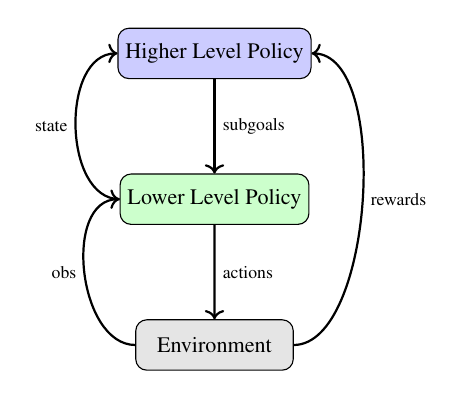
\begin{tikzpicture}[scale=0.8, transform shape, node distance=1.5cm]
                % Higher level policy
                \node[draw, rounded corners, fill=blue!20, minimum width=2.5cm, minimum height=0.8cm] (high) {Higher Level Policy};
                
                % Lower level policy
                \node[draw, rounded corners, fill=green!20, minimum width=2.5cm, minimum height=0.8cm, below=of high] (low) {Lower Level Policy};
                
                % Environment
                \node[draw, rounded corners, fill=gray!20, minimum width=2.5cm, minimum height=0.8cm, below=of low] (env) {Environment};
                
                % Arrows
                \draw[->, thick] (high) -- node[right, font=\footnotesize] {subgoals} (low);
                \draw[->, thick] (low) -- node[right, font=\footnotesize] {actions} (env);
                \draw[->, thick] (env) to[out=180,in=180] node[left, font=\footnotesize] {obs} (low);
                \draw[->, thick] (low) to[out=180,in=180] node[left, font=\footnotesize] {state} (high);
                \draw[->, thick] (env) to[out=0,in=0, looseness=0.7] node[right, font=\footnotesize] {rewards} (high);
            \end{tikzpicture}
        \end{column}
    \end{columns}
\end{frame}

\begin{frame}
    \frametitle{Contributions}
    
    \begin{itemize}
        \item \hieros \citep{mattes2024hieroshierarchicalimaginationstructured}: A Hierarchical RL agent with multi-layered world models enabling long-term planning and precise predictions
        \item S5WM: A world model using S5 layers with efficient design and internal state access
        \item ETBS: $O(1)$ time complexity experience sampling method
        \item SOTA performance on Atari100k benchmark
        \item Comprehensive ablation studies validating their hierarchical approach
    \end{itemize}
\end{frame}

\begin{frame}
    \begin{figure}
        \centering
        \includegraphics[width=0.52\textwidth]{assets/hierarchical_structure.png}
        \hspace{0.3cm}
        \includegraphics[width=0.35\textwidth]{assets/s5_arch.png}
        \vspace{-0.1cm}
        \caption{On the left: Hierarchical subactor structure of \hieros. Each layer of the hierarchy learns its own latent state world model and interacts with the other layers via subgoal proposal. The action outputs of each actor/critic is the subgoal input of the next lower layer. The output of the lowest level actor/critic is the actual action in the real environment. On the right: Training and imagination procedure of the S5WM. \hieros uses a stack of S5 blocks with their architecture shown above.}
        \label{fig:hieros_structure}
    \end{figure}
\end{frame}

\begin{frame}
    \frametitle{Overall Architecture}

    \begin{itemize}
        \item \textbf{Hierarchy of subactors}: $L\!+\!1$ levels (indexed $i=0,\dots,L$)
        \begin{itemize}
            \item Level 0 (the "worker") acts in the real environment, taking primitive actions
            \item Higher levels ($i\ge1$) output \textit{subgoals} for the level immediately below ($i-1$)
        \end{itemize}
        \item \textbf{Time-scale separation}: Each higher level holds its subgoal constant for $k$ lower-level steps
    \end{itemize}
    
    At each level $i$, three modules:
    \begin{enumerate}
        \item A \textit{world model} $w^i_{\theta}$
        \item An \textit{actor--critic} $\pi^i_\phi$
        \item A \textit{subgoal autoencoder} $g^i_\psi$
    \end{enumerate}
\end{frame}

\begin{frame}
    \frametitle{World Model \& Imagined Rollouts}
        
    Each subactor trains its own S5-style world model $w^i_\theta$ to predict future latent states:
    \begin{itemize}
        \item \textbf{Input:} either real env.\ observations (for $i=0$) or the lower-level's imagined states aggregated over $k$ steps (for $i\ge1$)
        \item \textbf{Usage:} the world model then \textit{imagines} trajectories, allowing actor--critic training without further environment calls
    \end{itemize}
            
\end{frame}

\begin{frame}
    \frametitle{Subgoal Autoencoder}
    
    The autoencoder at level $i$ compresses high-dimensional model states into a small discrete space of subgoals:
    
    \begin{align*}
        &\text{Encoder:} \quad g_t \sim p_\psi(g_t \mid h_t)\,,\\
        &\text{Decoder:} \quad \hat h_t = f_\psi(g_t)\approx h_t.
    \end{align*}
    
    \begin{itemize}
        \item $h_t$ is the \textit{deterministic} part of the world model state
        \item The discrete code $g_t$ is much lower-dimensional than $h_t$
    \end{itemize}
    
    \textbf{Training loss} (a standard $\beta$-VAE):
    
    \begin{align*}
        \mathcal{L}_\psi = \|f_\psi(z) - h_t\|_2 + \beta\,\mathrm{KL}\bigl[p_\psi(g_t\mid h_t)\,\big\|\,q(g_t)\bigr],
    \end{align*}
    
    where $q(g)$ is a uniform prior over codes.
            
\end{frame}

\begin{frame}
    \frametitle{Action \& Policy Inputs}
            
    At each time step the actor $\pi^i_\phi$ receives:
    
    \begin{align*}
        a_t \sim \pi^i_\phi\bigl((h_t,z_t),\,g_t,\,r_t,\,c_t,\,H\bigl(p_\theta(z_t\mid m_t)\bigr)\bigr).
    \end{align*}
    
    \begin{itemize}
        \item $(h_t,z_t)$ - full latent state from the world model
        \item $g_t$ - the \textit{current} subgoal
        \item $r_t$ - the reward signal at level $i$
        \item $c_t$ - continue flag (e.g.\ episode not done)
        \item $H\bigl(p_\theta(z_t\mid m_t)\bigr)$ - the entropy of the stochastic latent
    \end{itemize}
\end{frame}

\begin{frame}
    \frametitle{Reward Composition}
            
    Each subactor maximizes a \textit{mixed} reward:
    
    \begin{align*}
        r = r_{\rm extr} + w_g\,r_g + w_{\rm nov}\,r_{\rm nov}
    \end{align*}
    
    where:
    \begin{itemize}
        \item \textbf{$r_{\rm extr}$} is the environment's raw reward (only nonzero at level 0)
        \item \textbf{Subgoal reward} $r_g$ measures alignment with the intended subgoal:
        \begin{align*}
            r_g = \frac{g_t^\top\,h_t}{\max\bigl(\|g_t\|,\|h_t\|\bigr)}
        \end{align*}
        \item \textbf{Novelty reward} $r_{\rm nov}$ is the reconstruction error:
        \begin{align*}
            r_{\rm nov} = \bigl\| h_t - g^i_{\psi}(h_t) \bigr\|_2
        \end{align*}
    \end{itemize}
\end{frame}

\begin{frame}
    \frametitle{Multilayered Hierarchical Imagination}
    
    \begin{itemize}
        \item \textbf{Multi-Level Interaction}
        \begin{itemize}
            \item \textbf{Level 1} observes \textit{all} of the worker's imagined states for $k$ steps, then proposes a new subgoal $g^1$
            \item \textbf{Level 2} does the same on level 1's imagined sequences, and so on
            \item Earlier works like Director only feed every $k$th state to the higher policy
        \end{itemize}
        
        \item \textbf{Explainability \& Visualization}
        \begin{itemize}
            \item Each subgoal code $g^i$ can be decoded back into a world-model latent
            \item Makes hierarchical decisions interpretable
        \end{itemize}
        
        \item \textbf{Why it works}
        \begin{itemize}
            \item \textbf{Time abstraction} via holding subgoals constant for $k$ steps
            \item \textbf{State abstraction} via compressing $h_t$ into a low-dimensional discrete code
            \item \textbf{Intrinsic motivation} from novelty and subgoal rewards
            \item \textbf{Scalability} to more than two levels
        \end{itemize}
    \end{itemize}

\end{frame}

\begin{frame}
    \frametitle{S5-based World Model (S5WM)}
    
    \begin{itemize}
        \item \textbf{Core Components} (at each hierarchical level):
        \begin{itemize}
            \item \textbf{Sequence model:} $(m_t, h_t) = f_\theta\bigl(h_{t-1},\,z_{t-1},\,a_{t-1}\bigr)$
            \item \textbf{Encoder:} $z_t \sim q_\theta\bigl(z_t \mid o_t\bigr)$ (depends only on $o_t$, enabling parallel computation)
            \item \textbf{Dynamics predictor:} $\hat z_t \sim p_\theta\bigl(\hat z_t \mid m_t\bigr)$ (used during imagination)
            \item \textbf{Reward \& Continue predictors:} $\hat r_t \sim p_\theta\bigl(\hat r_t\mid h_t, z_t\bigr)$, $\hat c_t \sim p_\theta\bigl(\hat c_t\mid h_t, z_t\bigr)$
            \item \textbf{Decoder:} $\hat o_t \sim p_\theta\bigl(\hat o_t\mid h_t, z_t\bigr)$
        \end{itemize}
        
        \item \textbf{Training vs. Imagination}
        \begin{itemize}
            \item \textbf{Training:} Uses posterior $z_t \sim q(z_t\!\mid o_t)$ from real observations
            \item \textbf{Imagination:} Samples $\hat z_t\sim p(\hat z_t\!\mid m_t)$ without real observations
        \end{itemize}
        
        \item \textbf{Advantages of S5}
        \begin{itemize}
            \item Parallel \& autoregressive processing
            \item Long-range memory via structured state-space kernels
            \item Linear (not quadratic) memory cost in sequence length
            \item Direct use of recurrent hidden state as world-model component
        \end{itemize}
        
        \item \textbf{Episode-Reset Mechanism}
        \begin{itemize}
            \item Binary continue flags $c_0,\dots,c_n$ passed to S5 blocks
            \item When $c_t=0$ (episode start), internal state $h_t$ resets to learned initial $h_0$
        \end{itemize}
    \end{itemize}
\end{frame}

\begin{frame}
    \frametitle{S5WM Loss Functions}
    
    All parts trained end-to-end under a DreamerV3-style loss:
    \begin{align*}
        \mathcal{L}(\theta) = \underbrace{\mathcal{L}_{\rm pred}}_{\text{reward, cont., obs.}} + \alpha_{\rm dyn}\,\underbrace{\mathcal{L}_{\rm dyn}}_{\text{KL}\bigl[\mathrm{sg}\,q\|p\bigr]} + \alpha_{\rm rep}\,\underbrace{\mathcal{L}_{\rm rep}}_{\text{KL}\bigl[q\|\mathrm{sg}\,p\bigr]}
    \end{align*}
    
    \begin{itemize}
        \item \textbf{Prediction loss}
        \begin{align*}
            \mathcal{L}_{\rm pred} = -\ln p_\theta(r_t\mid h_t,z_t) -\ln p_\theta(c_t\mid h_t,z_t) -\ln p_\theta(o_t\mid h_t,z_t)
        \end{align*}
        
        \item \textbf{Dynamics loss}
        \begin{align*}
            \mathcal{L}_{\rm dyn} = \max\!\Bigl(1,\;\mathrm{KL}\bigl[\mathrm{sg}(q_\theta(z_t\!\mid o_t))\;\big\|\;p_\theta(z_t\!\mid m_t)\bigr]\Bigr)
        \end{align*}
        
        \item \textbf{Representation loss}
        \begin{align*}
            \mathcal{L}_{\rm rep} = \max\!\Bigl(1,\;\mathrm{KL}\bigl[q_\theta(z_t\!\mid o_t)\;\big\|\;\mathrm{sg}(p_\theta(z_t\!\mid m_t))\bigr]\Bigr)
        \end{align*}
    \end{itemize}
\end{frame}

\begin{frame}
    \frametitle{Efficient Time-balanced Sampling (ETBS)}

    \textbf{Problem:} Uniform sampling from growing replay buffer leads to imbalance
    \begin{itemize}
        \item Older entries (small index $i$) get oversampled
        \item Recent experiences are under-represented
    \end{itemize}
    
    \textbf{Quantifying the imbalance:}
    \begin{itemize}
        \item Expected draw count for entry $x_i$ after $n$ samplings:
        \begin{align*}
            \mathbb{E}[N_{x_i}] = \sum_{k=i}^{n}\frac{1}{k} = H_n - H_{i-1} \approx \ln(n) - \ln(i-1)
        \end{align*}
        \item Normalized probability:
        \begin{align*}
            p_i = \frac{\mathbb{E}[N_{x_i}]}{n} \approx \frac{\ln(n) - \ln(i)}{n}
        \end{align*}
    \end{itemize}

    \textbf{Solution}, from Imbalanced to Uniform via the CDF:

    \begin{itemize}
        \item \textbf{Key insight (Probability Integral Transform):} If $u\sim p(i)$ and $v = \mathrm{CDF}_p(u)$, then $v$ is uniformly distributed on $[0,1]$
        \item \textbf{Practical implementation:}
        \begin{itemize}
            \item Precompute the CDF of $p(i) \approx (\ln n - \ln i)/n$
            \item To sample: draw uniform $u\in[0,1]$, then compute $i = \mathrm{CDF}_p^{-1}(u)$
            \item This remaps the skewed distribution back to (nearly) uniform
        \end{itemize}
    \end{itemize}


\end{frame}

\begin{frame}
    \frametitle{ETBS Temperature-controlled Interpolation}
    
    \textbf{Temperature-controlled interpolation:}
    \begin{align*}
        p_{\rm ETBS}(i) = \tau\,\underbrace{\mathrm{CDF}_p\bigl(p(i)\bigr)}_{\text{"uniformized"}} + (1-\tau)\,p(i)
    \end{align*}
    where $\tau \in [0,1]$ controls uniformity vs. original bias ($\tau=0.3$ in practice)
    
    \textbf{Constant-time implementation:}
    \begin{itemize}
        \item Precompute lookup table for $\mathrm{CDF}_p$ over $i=1,\dots,n$
        \item Sampling via table lookup or binary search to invert CDF
        \item All steps run in $O(1)$ time per sample
    \end{itemize}
    
    \textbf{Benefits:}
    \begin{itemize}
        \item Balances recency and coverage
        \item Light bias toward older transitions improves stability
        \item $O(1)$ efficiency vs. $O(n)$ in prior time-balanced methods
    \end{itemize}
\end{frame}

\begin{frame}
    \frametitle{Experiments - Summary}
    
    \begin{itemize}
        \item \textbf{Setup:} Evaluated on Atari100k benchmark (25 games, 100k steps)
        \item Compared against SimPLe and imagination-based methods (TWM, IRIS, DreamerV3)
        \item \textbf{Results:} New state-of-the-art in mean/median human-normalized scores
        \begin{itemize}
            \item Matches or beats other methods on 9 of 25 games
            \item Trains in $\sim$14h per game (comparable to DreamerV3/TWM, faster than IRIS)
        \end{itemize}
        \item \textbf{Strengths:} Excels in games with shifting dynamics across levels
        \begin{itemize}
            \item Hierarchical subgoals direct exploration effectively
            \item Examples: Frostbite, James Bond, PrivateEye
        \end{itemize}
        \item \textbf{Limitations:} Weaker on simple-dynamics games (Breakout, Pong)
        \begin{itemize}
            \item S5WM struggles with uniform dynamics
            \item Hierarchy less beneficial when subgoals aren't informative
        \end{itemize}
        \item \textbf{Analysis:} S5WM better models long-term, shifting dynamics
        \begin{itemize}
            \item Successfully predicts level transitions in complex games
            \item Trade-off between model size and environment complexity
        \end{itemize}
    \end{itemize}
\end{frame}

\begin{frame}
    \frametitle{Experiments - Atari100k Results}
    
    \begin{table}[h]
      \centering
      \resizebox{0.9\textwidth}{!}{
      \begin{tabular}{l|rr|rrrrr}
          Task & Random & Human & SimPLe & TWM & IRIS & DreamerV3 & Hieros \\\hline
          Alien           & 228          & 7\,128           & 617                  & 675        & 420       & \textbf{959}          & 828 \\
          Amidar          & 6            & 1\,720           & 74                   & 123         & 143          & 139        & 127 \\
          Assault         & 222          & 742            & 527                  & 683          & 1\,524        & 706       & \textbf{1\,764} \\
          Asterix         & 210          & 8\,503           & \textbf{1\,128}        & 1\,117        & 854       & 932         & 899 \\
          BankHeist       & 14           & 753            & 34                   & 467        & 53        & \textbf{649}         & 177 \\
          Battle Zone     & 2\,360         & 37\,188          & 4\,031                 & 5\,068        & 13\,074         & 12\,250          & \textbf{15\,140} \\
          Boxing          & 0            & 12             & 8                    & 78         & 70         & \textbf{78}        & 65 \\
          Breakout        & 2            & 30             & 16                   & 20         & \textbf{84}          & 31       & 10 \\
          Chop.Command    & 811          & 7\,388           & 979                  & \textbf{1\,697}          & 1\,565       & 420          & 1\,475 \\
          CrazyClimber    & 10\,780        & 35\,829          & 62\,584                & 71\,820          & 59\,324          & \textbf{97\,190}           & 50\,857 \\
          DemonAttack     & 152          & 1\,971           & 208                  & 350        & \textbf{2\,034}       & 303         & 1\,480 \\
          Freeway         & 0            & 30             & 17                   & 24       & \textbf{31}       & 0       & \textbf{31} \\
          Frostbite       & 65           & 4\,335           & 237                  & 1\,476       & 259       & 909        & \textbf{2\,901} \\
          Gopher          & 258          & 2\,412           & 597                  & 1\,675          & 2\,236       & \textbf{3\,730}        & 1\,473 \\
          Hero            & 1\,027         & 30\,826          & 2\,657                 & 7\,254         & 7\,037       & \textbf{11\,161}        & 7\,890 \\
          JamesBond       & 29           & 303            & 100                  & 362      & 463         & 445        & \textbf{939} \\
          Kangaroo        & 52           & 3\,035           & 51                   & 1\,240         & 838        & 4\,098          & \textbf{6\,590} \\
          Krull           & 1\,598         & 2\,666           & 2\,205                 & 6\,349         & 6\,616        & 7\,782       & \textbf{8\,130} \\
          KungFuMaster    & 258          & 22\,736          & 14\,862                & \textbf{24\,555}          & 21\,760           & 21\,420          & 18\,793 \\
          Ms.Packman      & 307          & 6\,952           & 1\,480                 & 1\,588         & 999          & 1\,327       & \textbf{1\,771} \\
          Pong            & -21          & 15             & 13                   & \textbf{18}         & 15         & \textbf{18}        & 5 \\
          PrivateEye      & 25           & 69\,571          & 35                   & 86         & 100        & 882         & \textbf{1\,507} \\
          Qbert           & 164          & 13\,455          & 1\,289                 & 3\,331        & 746       & \textbf{3\,405}       & 770 \\
          RoadRunner      & 12           & 7\,845           & 5\,641                 & 9\,109          & 9\,615       & 15\,565       & \textbf{16\,950} \\
          Seaquest        & 68           & 42\,055          & 683         & \textbf{774}        & 661        & 618       & 560 \\\hline &&&& \\[-2ex]
          Mean            & 0            & 100            & 34                   & 96         & 105        & 112        & \textbf{120} \\ 
          Median          & 0            & 100            & 11                   & 50         & 29         & 49         & \textbf{56} \\
          IQM            & 0            & 100            & 13                   & 46         & 50        & N/A        & \textbf{53} \\ 
          Optimality Gap          & 100            & 0            & 73                   & 52         & 51         & N/A         & \textbf{49} \\
      \end{tabular}
      }
    \end{table}
\end{frame}

\begin{frame}
    \frametitle{Experiments - Rewards Graph}

    \begin{figure}[t]
        \centering
        \includegraphics[width=0.65\textwidth]{assets/rewards_vert.png}
        \vspace{-0.1cm}
        \caption{Extrinsic, subgoal, and novelty rewards per step for Krull (top) and Breakout (bottom) for the lowest level subactor.
        \vspace{-0.05cm}}
        \label{fig:rewards}
    \end{figure}
\end{frame}

\begin{frame}
    \frametitle{Experiments - Reward Analysis}

    Analysis of partial rewards ($r_{extr}$, $r_{nov}$, and $r_{sg}$) for the lowest level subactor in Breakout and Krull reveals:
    \begin{itemize}
        \item Breakout: Sparse extrinsic rewards provide little guidance for score improvement
        \begin{itemize}
            \item Subactor relies heavily on higher-level subgoals
            \item Strict adherence to subgoals hinders performance
        \end{itemize}
        \item Krull: More frequent extrinsic rewards offer clearer direction
        \begin{itemize}
            \item Subactor treats higher-level subgoals as flexible hints
            \item Leads to better overall performance
        \end{itemize}
    \end{itemize}
\end{frame}

\begin{frame}
    \frametitle{Experiments - RSSM vs. S5WM}

    \begin{figure}[t] 
        \centering
        \includegraphics[width=0.65\textwidth]{assets/rssm_s5_vert.png}
        \vspace{-0.1cm}
        \caption{World model losses for the S5WM and RSSM for Krull and Breakout. The S5WM is able to achieve an overall lower world model loss compared to the RSSM for Krull, while those roles are reversed for Breakout.
        \vspace{-0.3cm}}
    \label{fig:losses}
    \end{figure}
\end{frame}

\begin{frame}
    \frametitle{Experiments - S5WM vs. RSSM Analysis}

    To directly compare our S5WM architecture with the RSSM used in DreamerV3, the S5WM was replaced with an RSSM and trained HIEROS on four different games:
    \begin{itemize}
        \item RSSM underperforms S5WM in Krull, Battle Zone, and Freeway
        \item RSSM slightly outperforms S5WM in Breakout
        \item S5WM achieves lower overall world model loss in Krull
        \item RSSM achieves lower loss in Breakout
    \end{itemize}

    \vspace{0.2cm}
    Key insights:
    \begin{itemize}
        \item S5WM excels in complex environments with substantial input distribution shifts
        \item RSSM performs better in simpler environments with stable input distributions
        \item The difference is particularly notable given Krull's higher absolute loss values
    \end{itemize}
\end{frame}


\end{document}